\section{Blast Algorithm}
\label{sec:introduction}

BLAST algorithm is used to search for similar parts of sequence between database and query. There are several implementations of BLAST based on their processing data: nucleotides having 4 letter alphabet and amino acids having 20 letters. The inputs to BLAST is two sequence - database, which consists of a huge amount of data, and a query, which is to be compared with database and find the similar parts of sequence. The output of algorithm are the degree(score) of similarity of the aligned parts and their corresponding location in the sequences. Each of matched pair in database and query is called a High Score Pair(HSP) and is of extreme importance for further biological computations. 
\\
\begin{figure}
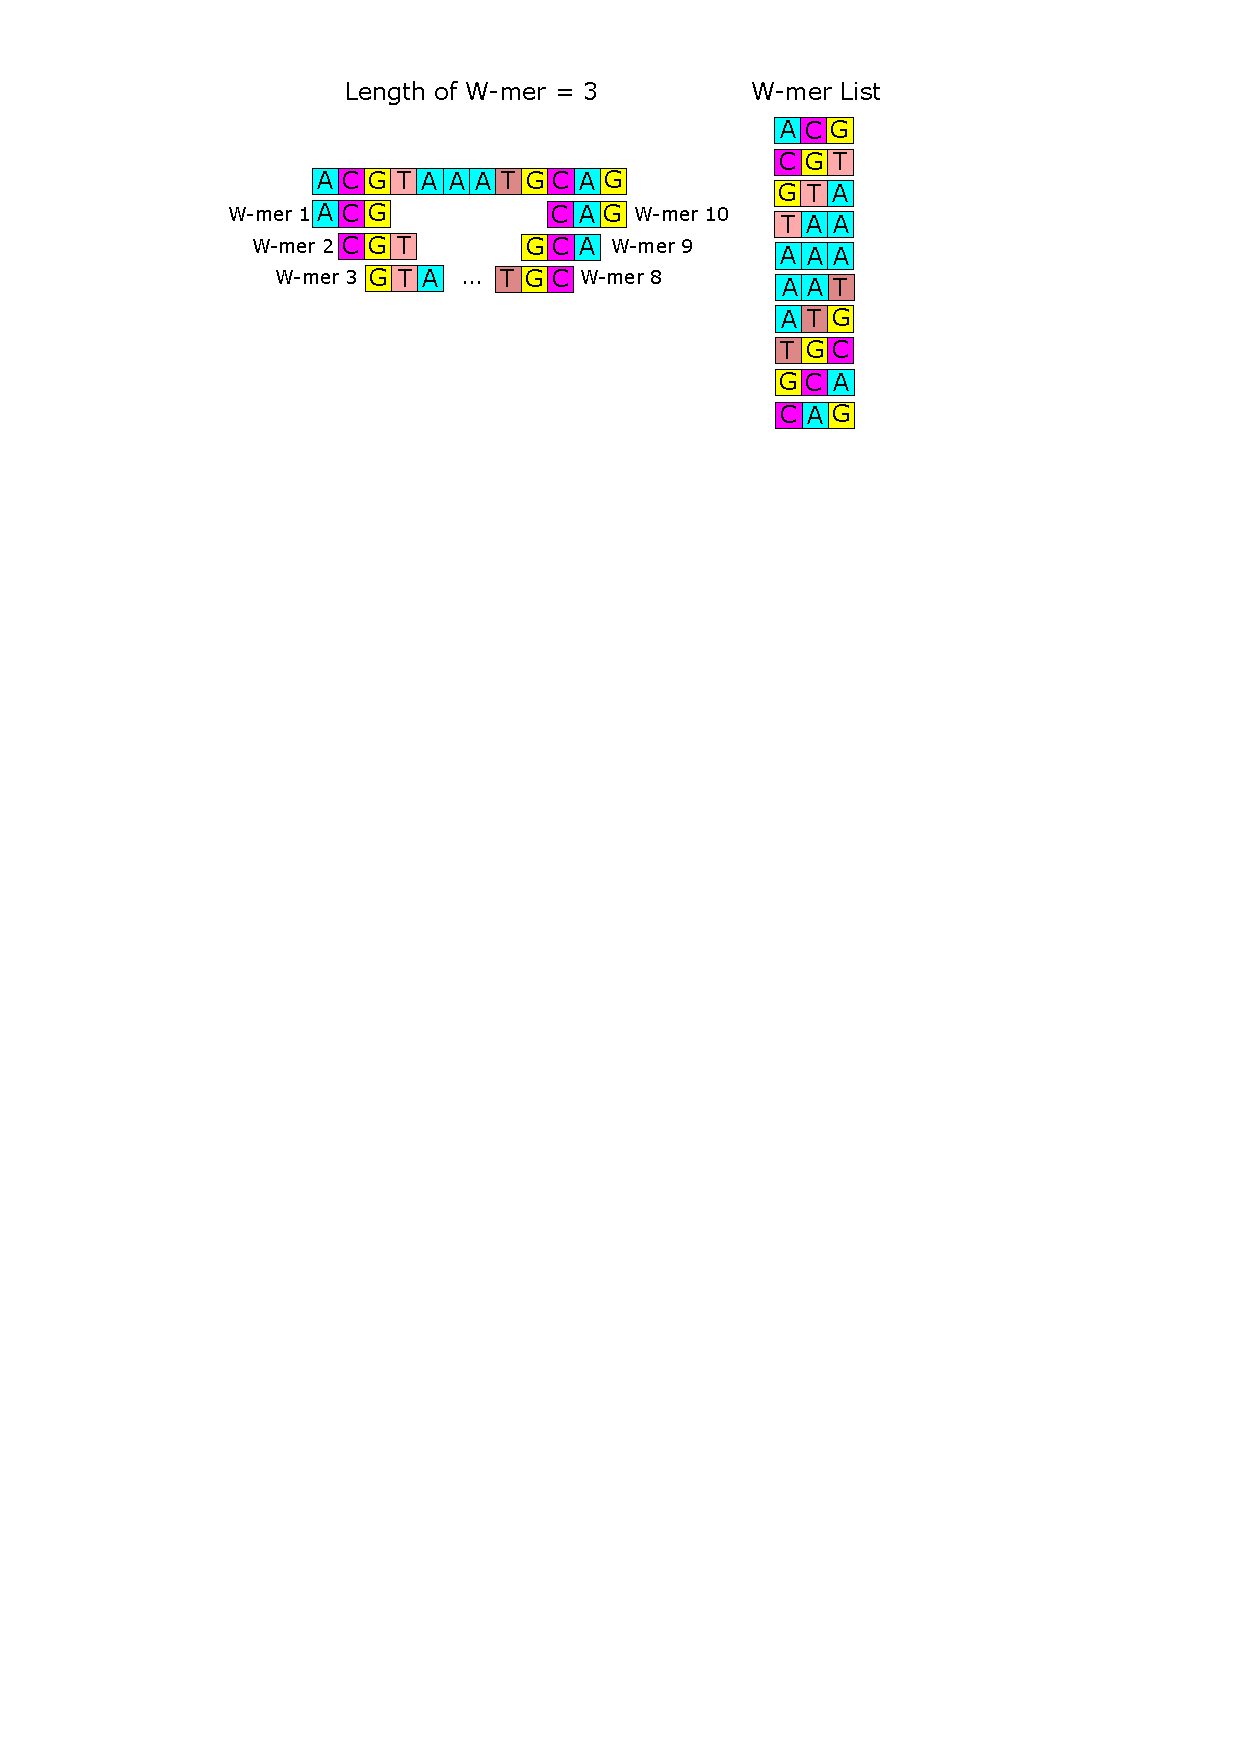
\includegraphics[width=\textwidth]{Figures/Algorithm1.pdf}
\caption{A figure caption is always placed below the illustration.
Please note that short captions are centered, while long ones are
justified by the macro package automatically.} \label{fig1}
\end{figure}
\begin{figure}
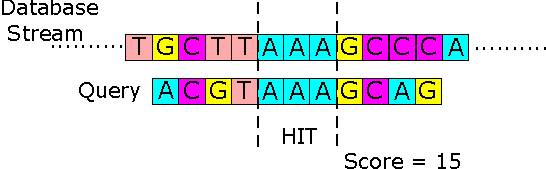
\includegraphics[width=\textwidth]{Figures/Algorithm2.pdf}
\caption{A figure caption is always placed below the illustration.
Please note that short captions are centered, while long ones are
justified by the macro package automatically.} \label{fig3}
\end{figure}
\begin{figure}
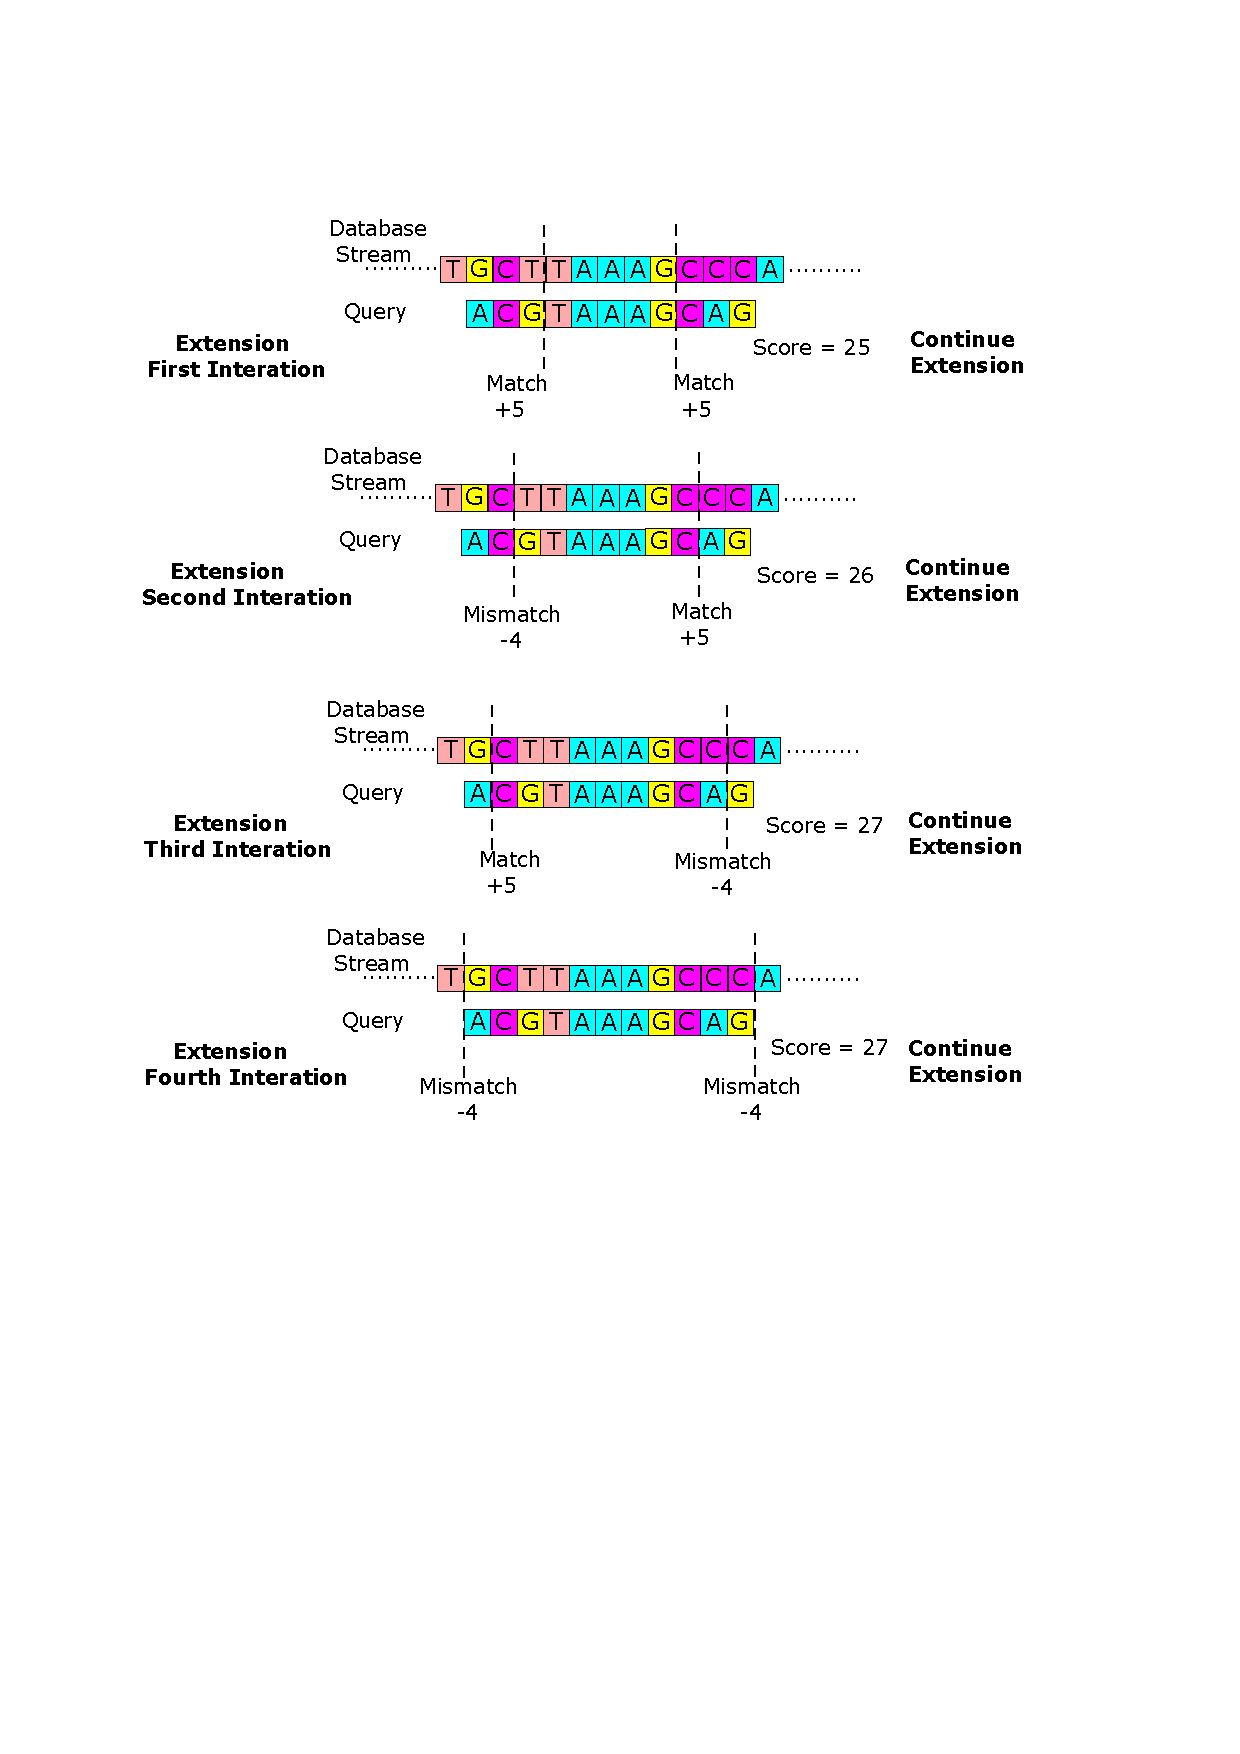
\includegraphics[width=\textwidth]{Figures/Algorithm3.pdf}
\caption{A figure caption is always placed below the illustration.
Please note that short captions are centered, while long ones are
justified by the macro package automatically.} \label{fig4}
\end{figure}